% Use only LaTeX2e, calling the article.cls class and 12-point type.

\documentclass[12pt]{article}

\usepackage{scicite}
\usepackage[utf8]{inputenc} %utf8 % lettere accentate da tastiera
\usepackage[english]{babel} % lingua del documento
\usepackage[T1]{fontenc} % codifica dei font
\usepackage[backend=bibtex,sorting=none, backref=true]{biblatex}
\usepackage{times}
\usepackage{amssymb}
\usepackage{amsmath}
\usepackage{graphicx}
\usepackage{subfigure}
\usepackage{caption}

\topmargin 0.0cm
\oddsidemargin 0.2cm
\textwidth 16cm 
\textheight 21cm
\footskip 1.0cm

\newenvironment{sciabstract}{%
\begin{quote} \bf}
{\end{quote}}


\renewcommand\refname{References and Notes}

\newcounter{problem}
\newcounter{solution}

\newcommand\Problem{%
	\stepcounter{problem}%
	\textbf{\theproblem.}~%
	\setcounter{solution}{0}%
}

\newcommand\TheSolution{%
	\textbf{Solution:}\\%
}

\newcommand\ASolution{%
	\stepcounter{solution}%
	\textbf{Solution \thesolution:}\\%
}

\parindent 0in
\parskip 1em

\newcounter{lastnote}
\newenvironment{scilastnote}{%
\setcounter{lastnote}{\value{enumiv}}%
\addtocounter{lastnote}{+1}%
\begin{list}%
{\arabic{lastnote}.}
{\setlength{\leftmargin}{.22in}}
{\setlength{\labelsep}{.5em}}}
{\end{list}}

\title{Machine Learning \\ \Large{Assignment 1: Neural Networks} \\[0.3em] \normalsize{Faculty of Informatics} \\ \normalsize{Università della Svizzera Italiana}}


\author {{Giorgia Adorni}	\\ \normalsize{giorgia.adormi@usi.ch}}


\date{\today}

\bibliography{scibib}

%%%%%%%%%%%%%%%%% END OF PREAMBLE %%%%%%%%%%%%%%%%

\begin{document} 

% Double-space the manuscript.
%\baselineskip24pt

\maketitle 

\section{The Perceptron}
\begin{figure}[h!]
	
	\begin{minipage}[c]{.5\textwidth}
		\centering
		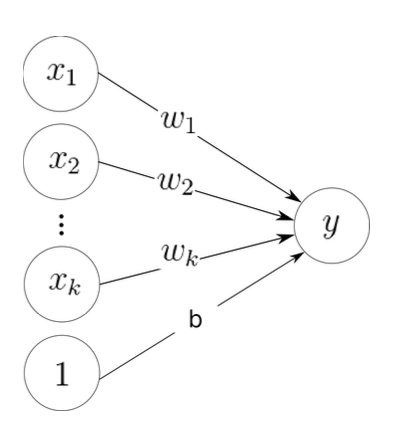
\includegraphics[width=.7\linewidth]{neuron.png}
		\captionof{figure}{The linear perceptron with single output}
		\label{fig:test1}
	\end{minipage}%
	~
	\begin{minipage}[c]{.5\textwidth}
		\centering
			\begin{tabular}{|c|c|c|c|}
				\hline
				$\overline{x}_{i,1}$ & $\overline{x}_{i,2}$ & $\overline{x}_{i,3}$ & $\hat{y}_i$ \\\hline
				-9         & -5         & 5          & 0                           \\\hline
				4          & -7         & -11        & 0                           \\\hline
				7          & 6          & -1         & 1                           \\\hline
				-9         & -5         & 4          & 1                           \\\hline
				-5         & -6         & -1         & 1                           \\\hline
				-4         & -4         & -8         & 0                           \\\hline
				5          & 7          & -9         & 1                           \\\hline
				2          & -4         & 3          & 0                           \\\hline
				-6         & 1          & 7          & 0                           \\\hline
				-10        & 6          & -7         & 1                          \\\hline
			\end{tabular}
			\captionof{table}{The training dataset}
			\label{tab:traind-dataset}
	
	\end{minipage}
\end{figure}

Before working on a neural network we will study the perceptron; a linear classifier
without an activation function or a very simple single layer network as given in Figure 1.
You are given a dataset of size $n: \mathcal{D} = \{(\overline{x}_1 ,\hat{y}_1),(\overline{x}_n ,\hat{y}_2),\dots , (\overline{x}_n ,\hat{y}_n)\}$, where input is represented as $k$-dimensional vectors $\overline{x}_i \in \mathbb{R}^k$, and the targets $\hat{y}_i \in \mathbb{R}$ are scalar. Assume bias term $b \in \mathbb{R}$ is not part of weight matrix $\underline{W} = [w_1,w_2,\dots,w_k]^T$.

\newpage

\Problem{What is the dimension of the output vector $\overline{y}$ if we assume a batch of input data in form $\underline{x} \in \mathbb{R}^{d \times k}$?}

\TheSolution {The output shape of the vector $\overline{y}$ is $d$. Given $d$ batch as input, the resulting output as the same dimension $d$.}

\Problem{Write down the vectorized equation for the forward pass, if input $\underline{x} \in \mathbb{R}^{d \times k}$ is batch of data, and $\overline{1}_d$ is a length $d$ long vector of ones (watch out for dimensions to match).}

\TheSolution {…}

\Problem{Write down the vectorized equation for the MSE of the perceptron.}

\TheSolution {…}

\Problem{Determine the derivative of the error function w.r.t weights \textit{Hint: $\frac{\partial \overline{x}^T\overline{x}}{\partial\overline{x}^T} = 2\overline{x}$}}

\TheSolution {…}

\Problem{Write down the equation of the weight update by gradient descent.}

\TheSolution {…}

\Problem{Suppose $k = 3\mbox{, }d =10$, with a batch of data given in Table 1. The initial weights are $w_1 = -0.1$, $w_2 = -0.3$, $w_3 = 0.2$ and the bias weight is $b = 2$. Compute the weights after one step of gradient descent with learning rate of $\eta = 0.02$ (report their value up to 2 decimal points). \textit{Hint: MATLAB/Octave/Python might come in handy here.}}

\TheSolution {…}

\Problem{Learning in multi-layer neural networks is usually done with help of two methods: back-propagation and gradient descent. Describe briefly what role in the learning process each of the two has (Should not be longer than $6$ lines).}

\TheSolution {…}

\printbibliography
\nocite{*}

\end{document}




















